\subsection{Indicadores Financieros}

Los indicadores financieros se basan en la comparación de dos valores esenciales dentro de los documentos internos de una empresa: balance general y presupuesto de la empresa. Gracias a los indicadores financieros y su interpretación, un negocio puede saber qué rumbo necesita tomar con base a datos históricos analizados. \cite{mundi_2022}

Dentro de los indicadores financieros tomados en cuenta fueron los siguientes:

\begin{itemize}
    \item \textbf{Razón corriente: } Permite determinar la capacidad que tiene la empresa para cubrir las deudas con activos que posee.
    
    \item \textbf{Nivel de endeudamiento total: } Determina el grado y la forma de participación de todos los acreedores dentro de la economía de la empresa.
    
    \item \textbf{Rentabilidad operacional: } : Este indicador permite evidenciar el porcentaje en que los ingresos recibidos fueron convertidos en beneficios después de pagar los costos operacionales.
    
    \item \textbf{Rentabilidad neta: } Distingue el nivel de ganancias que se obtiene con respecto a las ventas netas una vez se paga costos fijos y variables.
    
    \item \textbf{Rentabilidad de patrimonio: } Muestra cual es el nivel de ganancia que tiene la empresa a partir de la inversión realizada por los accionistas.
    
    \item \textbf{Rentabilidad del activo:} Es una medida de la rentabilidad que tiene los activos adquiridos por la empresa, los cuales generan ganancias durante un periodo de tiempo
\end{itemize}

En la tabla \ref{indicadores} se proyectan los indicadores a 5 años.

\vspace{2mm}
\begin{minipage}{0.9\textwidth}
\centering
\captionof{table}[{Indicadores financieros}]{ Indicadores financieros}
\label{indicadores}
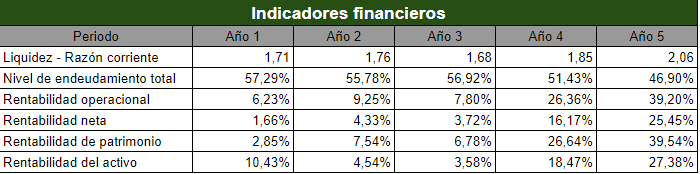
\includegraphics[width=0.9\textwidth]{Images/indicadoresFinancieros.png}
\fnote{Nota. \textup{Fuente : Autores}}
\end{minipage}

Por otro lado se tomaron los indicadores financieros VAN, TIR y relación costo-beneficio con el fin de demostrar viabilidad de inversión que tienen los accionistas. Los resultados obtenidos de flujo de caja se tienen en cuenta para los datos  ilustrados en la tabla \ref{flujoLibre}.

\vspace{2mm}
\begin{minipage}{0.9\textwidth}
\centering
\captionof{table}[{Flujo de caja libre
}]{ Flujo de caja libre
}
\label{flujoLibre}
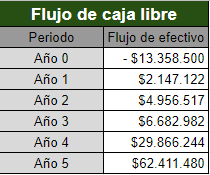
\includegraphics[\textwidth]{Images/flujoCajaLibre.png}
\fnote{Nota. \textup{Fuente : Autores}}
\end{minipage}


Teniendo en cuenta la tasa interna de oportunidad, que es la tasa de rendimiento mínimo que se esperaría recibir por parte de los accionistas, se construye de manera subjetiva asignándole un valor del 10\% para compensar la inversión realizada.

En la tabla \ref{vanTIR} se ilustran los resultados que la inversión realizada se recupera después de 5 años superando en \$56862412, logrando multiplicar por mas de 5 veces el capital invertido con una tasa interna de retorno del 66.27\%.

\vspace{2mm}
\begin{minipage}{0.9\textwidth}
\centering
\captionof{table}[{VAN, TIR y RBC}]{ VAN, TIR y RBC}
\label{vanTIR}
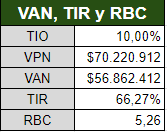
\includegraphics[\textwidth]{Images/vanTIR.png}
\fnote{Nota. \textup{Fuente : Autores}}
\end{minipage}

Revisando los resultados del análisis financiero se observa que el proyecto tiene viabilidad en esta área y depende del atractivo hacia futuros inversionistas el éxito de esta, con el fin de poder adquirir mayor capacidad en el mercado competitivo con una gran demanda para esta área de oportunidad. El VAN y TIR resultaron positivos junto con la mayor liquidez ilustrada en la tabla de proyección de incremento de ventas deduce que la empresa tendrá mejor y mayor liquidez junto un nivel de endeudamiento con tendencia a la baja y una rentabilidad con posibilidad de comportamiento exponencial en el transcurso de los años.